\documentclass{article}
\usepackage{setspace}
\usepackage{amsmath}
\usepackage{xcolor}
\usepackage{tikz}
\usepackage{hyperref}
\usepackage{tabularx}
\usepackage{graphicx}
\usepackage{amssymb}
\usepackage{listings}
\usepackage[margin=1in]{geometry}
\usepackage{xepersian}
\settextfont{Yas}
% Fixture for Xepersian 23 bug of setting persian math digit fonts
\ExplSyntaxOn\cs_set_eq:NN\etex_iffontchar:D\tex_iffontchar:D\ExplSyntaxOff
\setmathdigitfont{Yas}
\onehalfspacing
\title{
	تمرین دوم هوش مصنوعی
}
\author{
	امیرحسین رجبی (۹۸۱۳۰۱۳)
}
\renewcommand{\labelenumi}{\alph{enumi})}
\lstset{
	language=Python, 
	basicstyle=\ttfamily, 
	tabsize=4, 
	frame=single,
	commentstyle=\itshape\color{lightgray},
	keywordstyle=\bfseries\color{blue},
	identifierstyle=\color{black},
	stringstyle=\color{red}, 
	numbers=left
}
\bibliographystyle{plain}
\hypersetup{
	colorlinks=true,
	linkcolor=blue,
	filecolor=blue,
	citecolor = black,      
	urlcolor=cyan,
}
\newcommand{\code}[1]{\lr{\lstinline|#1|}}
\begin{document}
	\maketitle
	\section*{
		سوال اول
	}
	\begin{enumerate}
		\item 
		معادل الگوریتم 
		\lr{Random walk}
		خواهد بود زیرا اگر $x$ تنها حالت جمعیت باشد، دو حالت والد همان $x$ خواهند بود و در نتیجه پس از
		\lr{Cross over}
		فرزند همان $x$ خواهد شد و با جهش در یکی از حروف $x$ به یکی از همسایه‌های $x$ خواهیم رفت که دقیقا همان قدم زن تصادفی است.
		
	\item 
	معادل الگوریتم 
	\lr{Hill Climbing}
	خواهد بود زیرا در واقع بهترین همسایه حالت فعلی را انتخاب می‌کنیم و سراغ آن می‌رویم.
	\item 
	اگر $k$ بزرگ شود الگوریتم به این صورت خواهد بود که بسیاری از حالات و همسایه‌های آنها مورد بررسی قرار می‌گیرند و شبیه 
	\lr{Brute force}
	می‌شود که دائما تعداد زیادی از بهترین‌ها را انتخاب و وجود حالت هدف را در آن ها بررسی می‌کند.
	\item 
	اگر دما همواره صفر باشد هیچ گاه به حالتی با ارزش کمتر نخواهیم رفت و دقیقا شبیه 
	\lr{Hill Climbing}
	رفتار می‌کند. (دقت کنید لازم است شظر خاتمه الگوریتم تغییر کند به این که هیچ همسایه بهتری وجود ندارد و اگرنه با شرط فعلی که صفر بودن $T$ است الگوریتم از حلقه خارج می‌شود و جواب تصادفی نخست را برمی‌گرداند.)
	\item
	الگوریتم به سرعت به یک مینیموم یا ماکسموم محلی همگرا می‌شود چرا که الگوریتم تنها در صورتی از تپه پایین خواهد آمد که
	$\Delta E$
	کوچک باشد (هم مرتبه $T$ باشد) و برای کاهش ارتفاع زیاد، ($-\Delta E$ بزرگ) عملیات پایین آمدن 
	\lr{Reject}
	شده و فقط با مشاهده همسایه‌ها با ارزش بزرگتر، از تپه بالا می‌رود در نتیجه به سرعت مانند 
	\lr{Hill Climbing}
	رفتار خواهد کرد. اگر $T$ ثابت باشد الگوریتم از ابتدا تنها زمانی سراغ پایین آمدن از تپه می‌رود که 
	$\Delta E$
	بسیار کوچک باشد یعنی حول همان جوابی که هست یا باقی می‌ماند یا سراغ جواب های بهتر می‌رود ولی خطر کاهش ارتفاع زیاد را به جان نمی‌خرد. تقریبا شبیه 
	\lr{Hill Climbing}
	عمل خواهد کرد.
	\end{enumerate}

	\section*{
		سوال دوم
	}
	\begin{enumerate}
		\item 
	 	همه جایگشت های $n$ کلمه خواهد بود. اگر $n$ کلمه متمایز باشند می‌شود $n!$ و اگر $i$ کلمه متمایز داشته باشیم و  تکرار هر کدام 
	 	$t_1, \dots , t_i$
	 	باشند برابر
	 	$\frac{n!}{t_1!t_2!\cdots t_n!}$
	 	خواهد بود.
	 	\item 
	 	یک نوع می‌توان همسایگی بین جملات تعریف کرد به این صورت که دو جمله همسایه باشند اگه جای دو کلمه آنها عوض شده باشد. مثلا جملات «این است مجازی ترم هوش مصنوعی» و «هوش مصنوعی است این ترم مجازی» همسایه جمله داده شده خواهند بود.
	 	\item 
	 	خیر زیرا اساسا الگوریتم 
	 	\lr{Hill Climbing}
	 	الگوریتمی
	 	\lr{Complete}
	 	نیست و ممکن است در مینیموم و ماکسیموم‌های محلی و فلات‌ها گیر کند و عملا هیچ‌گاه به نقطه بهین سراسری نرسد.
	 	\item 
	 	اگر دو جمله «این است مجازی ترم هوش مصنوعی» و «هوش مصنوعی است این ترم مجازی» در مرحله
	 	\lr{Selection}
	 	به عنوان والد انتخاب شده باشند، نتیجه عملیات 
	 	\lr{Cross over}
	 	با محل شکست پس از دومین کلمه، می‌تواند فرزندان روبرو باشد: «این است این ترم مجازی» و «هوش مصنوعی است مجازی ترم هوش مصنوعی».
	 	
	\end{enumerate}
	\section*{
	گزارش پیاده سازی الگوریتم 
	\lr{Simulated Annealing}
}
برای هر حالت مسئله یا ترتیب دهی رئوس مانند $v_1, v_2, \dots, v_n$، تابع هدف $f$ برابر تعداد یال‌هایی مانند $v_i \rightarrow v_j$ خواهد بود که $i < j$؛ یعنی تعداد یال‌ها در جهت ترتیب نهایی. هدف بیشینه کردن تابع $f$ است. به وضوح بیشترین مقدار $f$ برابر تعداد یال‌های گراف خواهد بود. همچنین همسایگی یک حالت مانند $v_1, v_2, \dots, v_n$ همه حالت‌هایی خواهند بود که با جابجایی $v_i$ و $v_j$ بدست آمده باشند؛ یعنی $v_1, \dots, v_j, \dots, v_i, \dots, v_n$ که $i < j$. در این صورت الگوریتم \lr{SA} را می‌توان برای محاسبه ترتیب توپولیژیکی گراف ورودی به کار برد.

تابع 
\code{read\_graph()}
گراف را از فایل خوانده و تعداد رئوس، تعداد یال‌ها و یک 
\code{dict}
بر می‌گرداند که هر راس مانند $u$ را به مجموعه (\code{set}) رئوسی نگاشت می‌کند که یالی جهت دار از $u$ به آنها وجود داشته باشد.

\begin{latin}
\begin{lstlisting}
def read_graph(file_name):
	with open(file_name) as f:
		lines = f.readlines()
		vertex_count = int(lines[0])
		edge_count = 0
		graph = {}
		for vertex in range(1, vertex_count + 1):
			graph[vertex] = set()
		for line in lines[1:]:
			x, y = map(int, line.split())
			edge_count += 1
			graph[x].add(y)
	return vertex_count, edge_count, graph
\end{lstlisting}
\end{latin}

تابع 
\code{val()}
مقدار تابع هدف را محاسبه می‌کند که پیاده سازی آن به صورت زیر است:
\begin{latin}
\begin{lstlisting}
def val(graph: dict, order: list):
	total = 0
	for i in range(len(order)):
		for j in range(i + 1, len(order)):
			if order[j] in graph[order[i]]:
				total += 1
	return total
\end{lstlisting}
\end{latin}
تابع 
\code{random\_successor\_and\_value(graph, current\_order, current\_value)}
با ورودی گرفتن گراف مسئله و حالت فعلی مقدار تابع هدف در حالت فعلی، یک حالت تصادفی از بین همسایه‌ها انتخاب می‌کند. در واقع به تصادف دو اندیس از ترتیب توپولیژیکی فرضی فعلی را انتخاب کرده و این دو راس را \lr{swap} می‌کند. برای بهبود سرعت الگوریتم دوباره از تابع 
\code{val()}
با پیچیدگی
$\mathcal{O}(n^2)$
برای محاسبه مقدار تابع هدف در حالت همسایه استفاده نشده است و به کمک مقدار فعلی تابع هدف با الگوریتمی از مرتبه 
$\mathcal{O}(n)$
مقدار $f$ حالت مجاور برگردانده می‌شود. در این الگوریتم تغییرات تابع $f$ روی رئوس بین 
$v_i$
و
$v_j$
در ترتیب توپولیژیکی محاسبه می‌شوند چرا که جابجایی این دو راس تاثیری در باقی رئوس و تغییر تابع $f$ به سبب آنها ندارد.
\begin{latin}
\begin{lstlisting}
def random_successor_and_value(graph: dict, current_order: list, 
							   current_value: int):
	i, j = sorted(random.sample(range(len(current_order)), k=2))
	delta = 0
	if current_order[i] in graph[current_order[j]]:
		delta = 1
	if current_order[j] in graph[current_order[i]]:
		delta = -1
	for k in range(i + 1, j):
		if current_order[i] in graph[current_order[k]]:
			delta += 1
		if current_order[j] in graph[current_order[k]]:
			delta -= 1
		if current_order[k] in graph[current_order[i]]:
			delta -= 1
		if current_order[k] in graph[current_order[j]]:
			delta += 1
	successor = current_order.copy()
	successor[i], successor[j] = successor[j], successor[i]
	return successor, current_value + delta
\end{lstlisting}
\end{latin}
در نهایت الگوریتم 
\lr{SA}
پیاده سازی شده است. در واقع یک ترتیب تصادفی برای شروع انتخاب شده و مقدرا تابع هدف به کمک تابع
\code{val()}
محاسبه شده است. در ادامه تابعی کمکی به نام
\code{decide()}
تعریف شده است که به احتمال $p$ (ورودی آن) مقدار 
\code{True}
و به احتمال
$1 - p$
مقدار
\code{False}
بر می‌گرداند. 
\begin{latin}
	\begin{lstlisting}
def simulated_annealing(vertex_count: int, graph: dict, temperature: int):
	current_order = [i for i in range(1, vertex_count + 1)]
	random.shuffle(current_order)
	current_value = val(graph, current_order)
	decide = lambda probability: random.random() < probability
	print(current_order, current_value)
	plot_data = [current_value]
	while temperature > 1e-6:
		successor, successor_value = random_successor_and_value(
			graph, 
			current_order, 
			current_value
		)
		delta = successor_value - current_value
		if delta >= 0 or decide(math.exp(delta / temperature)):
			current_order = successor
			current_value = successor_value
		temperature *= 0.9
		plot_data.append(current_value)
	return current_order, current_value, plot_data
	\end{lstlisting}
\end{latin}
مابقی الگوریتم مانند الگوریتم ذکر شده در شکل پنجم از فصل چهارم کتاب پیاده سازی شده است. نمودار تابع هدف (\code{current\_value}) براساس \lr{iteration}های الگوریتم به ازای بک بار اجرای آن روی ورودی نمونه داده شده به صورت زیر است: 

\begin{center}
	\begin{latin}
\begin{tabular}{|c|c|c|}
	\hline
	& \code{goal\_function} & \code{total\_edge\_count} \\
	\hline
	\code{initial\_order} & 20 & 54 \\
	\hline
	\code{goal\_order} & 47 & 54 \\
	\hline
\end{tabular}
\end{latin}
\end{center}

\begin{figure}[h]
	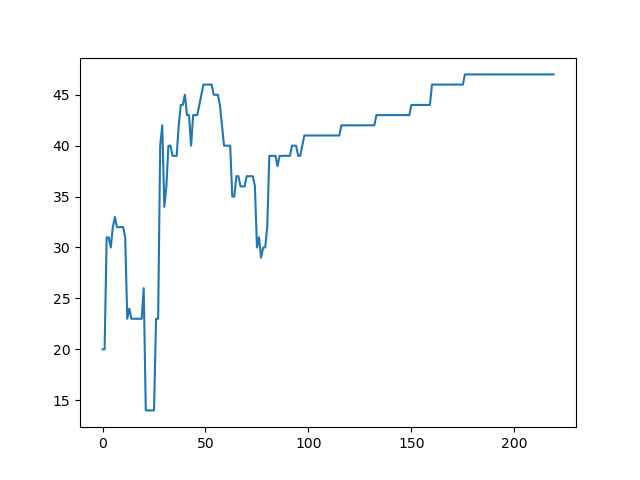
\includegraphics{simulated-annealing/fig}
	\caption{
	نمودار تابع هدف (\code{current\_value}) براساس \lr{iteration}ها
}
\end{figure}
\section*{
گزارش پیاده سازی
\lr{Genetic Algorithm}
}
تابع 
\lr{fitness}
این الگوریتم بسیار شبیه تابع هدف الگوریتم
\lr{SA}
 است یعنی اگر برای ترتیب 
$v_1, v_2, \dots, v_n$
از رئوس مقدار تابع $g$ برابر تعداد یال‌هایی مانند
$v_i \rightarrow v_j$
باشد که $i < j$ و همچنین $m$ تعداد کل یال‌های گراف و $c$ ضریب ثابتی باشد مقدار تابع 
\lr{fitness}
این مسئله برابر
$f = e^{\frac{gc}{m}}$
خواهد بود؛ یعنی بیشینه مقدار $f$ زمانی خواهد بود که 
$g = m$
باشد و در نتیجه
$e^c$
خواهد بود. دقت کنید رشد $f$ بر حسب $g$ نمایی است و این موجب همگرایی سریعتر الگوریتم می‌شود چرا که احتمال انتخاب والد‌هایی که $f$ بزرگتری دارند بالاتر می‌رود.

مانند الگوریتم
\lr{SA}
 که همسایه از طریق جابجایی دو راس انجام می‌شد، جهش یک کروموزوم با جابجایی تصادفی دو ژن انجام می‌شود. همچنین برای تولید فرزندان از تکنیکی مشابه کتاب استفاده می‌شود اما دو تفاوت وجود دارد: اول اینکه از هر دو والد یک فرزند تولید می‌شود. دوم اینکه برای تولید فرزندان معتبر (جایگشت رئوس گراف باشند) یک نقطه شکست به صورت تصادفی از کروموزوم والد اول انتخاب شده و ژن‌ها تا نقطه شکست از والد اول در فرزند کپی می‌شوند سپس ژن‌های باقی مانده از والد اول با توجه به ترتیب آنها در کروموزم والد دوم در ادامه کروموزوم فرزند کپی می‌شوند. به عنوان مثال اگر 
 $\textcolor{red}{p_1 = [2, 7, 1, 4, 5, 3, 6]}$
 کروموزوم والد اول و 
 $\textcolor{blue}{p_2 = [6, 7, 5, 1, 2, 4, 3]}$
 کروموزوم والد دوم باشد و محل شکست بعد از ژن سوم باشد در این صورت کروموزوم فرزند به صورت
 $c = [\textcolor{red}{2, 7, 1, } \, \textcolor{blue}{6, 5, 4, 3}]$
 خواهد بود. در این پیاده سازی جمعیت همواره ثابت و در ورودی سازنده کلاس 
 \code{GeneticAlgorithm}
 داده‌ می‌شود. همچنین متناسب تابع 
 \lr{fitness}
 احتمال‌هایی به کروموزوم‌های هر نسل نسبت داده می‌شود و برای تولید هر فرزند دو والد با این وزن‌های احتمالی انتخاب می‌شوند. (مشابه الگوریتم کتاب) واضح است که چون تابع 
  \lr{fitness}
  رشد نمایی دارد، شرط بقا ارضا شده و کروموزوم‌ها با کمترین مقدار تابع برازش احتمال بسیار کمی برای انتخبا به عنوان والد را دارند. از پارامترهای دیگر که ورودی سازنده کلاس 
   \code{GeneticAlgorithm}
   است احتمال جهش هر کروموزوم است ای همان درصد جمعیتی که جهش می‌یابند. برای توقف حلقه اصلی الگوریتم اولین شرط پیدا شدن هدف و دومین شرط گذشت زمان خاصی است که به عنوان ورودی به سازنده کلاس 
   \code{GeneticAlgorithm}
   داده شده است.
   
   با این توضیحات، پیاده سازی فعلی با جمعیت اولیه 1000 و احتمال جهش 
   $0.3$
   و لیمیت زمانی 2 ثانیه و فاکتور 
   $c = 30$
   در تابع برازش ($f = e^{\frac{gc}{m}}$) در همه اجرا‌ها می‌تواند حداقل ۵۳ یال از ۵۴ یال گراف را در جهت 
   \lr{topological order}
   قرار دهد و همچنین اغلب بعد از نسل هشتم این پایخ را بدست می‌آورد. در حدود ۵۰ نسل نیز در مدت ۲ ثانیه بررسی می‌شوند.
   به وضوح در مقایسه با الگوریتم
   \lr{SA}
   که بعد از 10000 گام پاسخ ۵۳ را روی ورودی نمونه بدست نمی‌آورد بسیار سریعتر و بهتر است.
   
   \begin{figure}[h]
   	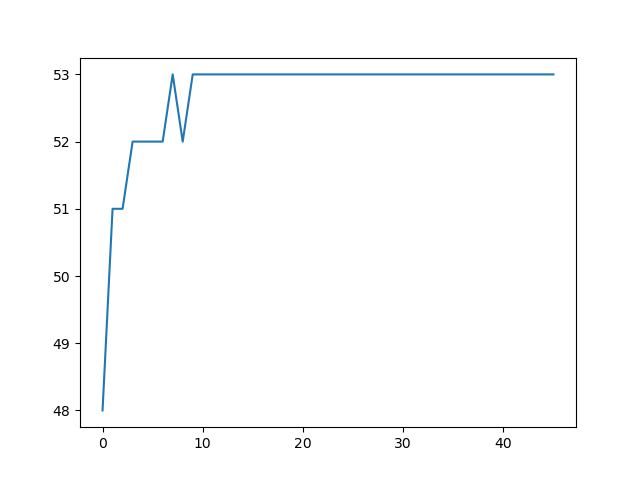
\includegraphics{genetic-algorithm/fig}
   	\caption{
   		نمودار تابع هدف براساس نسل‌ها
   	}
   \end{figure}
\end{document}